\documentclass[a4paper, 11pt]{article}
\usepackage{comment}
\usepackage{lipsum} 
\usepackage{fullpage} %cambiar margen
\usepackage[a4paper, total={7in, 10in}]{geometry}

\usepackage{amssymb,amsthm} 
\usepackage{amsmath}
\newtheorem{theorem}{Theorem}
\newtheorem{corollary}{Corollary}
\usepackage{graphicx}
\usepackage{tikz}
\usetikzlibrary{arrows}
\usepackage{verbatim}
%\usepackage[numbered]{mcode}
\usepackage{float}
\usepackage{tikz}
\usetikzlibrary{shapes,arrows}
\usetikzlibrary{arrows,calc,positioning}
\usepackage{mathpazo} %tipo de letra 
\usepackage[utf8]{inputenc} %codificación
\usepackage[T1]{fontenc} %digitación de tildes y ñ
\usepackage[spanish]{babel} %paquete de soporte español

\tikzset{
	block/.style = {draw, rectangle,
		minimum height=1cm,
		minimum width=1.5cm},
	input/.style = {coordinate,node distance=1cm},
	output/.style = {coordinate,node distance=4cm},
	arrow/.style={draw, -latex,node distance=2cm},
	pinstyle/.style = {pin edge={latex-, black,node distance=2cm}},
	sum/.style = {draw, circle, node distance=1cm},
}
\usepackage{xcolor}
\usepackage{mdframed}
\usepackage[shortlabels]{enumitem}
\usepackage{indentfirst}
\usepackage{hyperref}

\usepackage{listings}
\lstset{literate=
  {á}{{\'a}}1
  {é}{{\'e}}1
  {í}{{\'i}}1
  {ó}{{\'o}}1
  {ú}{{\'u}}1
  {Á}{{\'A}}1
  {É}{{\'E}}1
  {Í}{{\'I}}1
  {Ó}{{\'O}}1
  {Ú}{{\'U}}1
  {ñ}{{\~n}}1
  {ü}{{\"u}}1
  {Ü}{{\"U}}1
}

\lstdefinestyle{customc}{
  belowcaptionskip=1\baselineskip,
  breaklines=true,
  frame=L,
  xleftmargin=\parindent,
  language=Python,
  showstringspaces=false,
  basicstyle=\footnotesize\ttfamily,
  keywordstyle=\bfseries\color{green!40!black},
  commentstyle=\itshape\color{purple!40!black},
  identifierstyle=\color{blue},
  stringstyle=\color{orange},
}

\lstdefinestyle{customasm}{
  belowcaptionskip=1\baselineskip,
  frame=L,
  xleftmargin=\parindent,
  language=[x86masm]Assembler,
  basicstyle=\footnotesize\ttfamily,
  commentstyle=\itshape\color{purple!40!black},
}

\lstset{escapechar=@,style=customc}



\renewcommand{\thesubsection}{\thesection.\alph{subsection}}

\newenvironment{problem}[2][Ejercicio]
{ \begin{mdframed}[backgroundcolor= red!50] \textbf{#1 #2} \\}
	{  \end{mdframed}}

% Define solution environment
\newenvironment{solution}
{\textcolor{blue}{\textbf{\textit{Solución:\\\noindent}}}}


\renewcommand{\qed}{\quad\qedsymbol}

\newcommand{\esp}[1]{\mathbb{E}\left[#1\right]} % The expected value
\newcommand{\var}[1]{\text{Var}\left(#1\right)} % The variance
\newcommand{\prob}[1]{\mathbb{P}\left(#1\right)} % The probability
\newcommand{\probi}[2]{\mathbb{P}_{#1}\left(#2\right)} % The probability with ind
\newcommand{\R}{\mathbb{R}} %The R set

% \\	
\begin{document}
	\noindent
	%%%%%%%%%%%%%%%%%%%%%%%%%%%%%%%%%%%%
	
	\begin{minipage}[b][1.2cm][t]{0.8\textwidth}
		\large\textbf{César Isaí García Cornejo} \hfill \textbf{Tarea 1}  \\
		cesar.cornejo@cimat.mx \hfill \\
		\normalsize Ciencia de Datos \hfill Semestre 3\\
	\end{minipage}
	
	\hspace{14.4cm}
	\begin{minipage}[b][0.03cm][t]{0.12\linewidth}
		
		\vspace{-2.2cm}
		%%%La Ruta depeendera de donde este alojado el main y la imagen
		
\includegraphics[scale=0.3]{Images/EscudoCimat.png}
	\end{minipage}
	
	\noindent\rule{7in}{2.8pt}
	
	%%%%%%%%%%%%%%%%%%%%%
	%%%%%%%%%%%%%%%%%%%%%%%%%%%%%%%%%%%%%%%%%%%%%%%%%%%%%%%%%%%%%%%%%%%%%%%%%%%%%%%%%%%%%%%%%%%%%%%%%%%%%%%%%%%%%%%%%%%
	% Problem 1
	%%%%%%%%%%%%%%%%%%%%%%%%%%%%%%%%%%%%%%%%%%%%%%%%%%%%%%%%%%%%%%%%%%%%%%%%%%%%%%%%%%%%%%%%%%%%%%%%%%%%%%%%%%%%%%%%%%%%%%%%%%%%%%%%%%%%%%%%
	\setlength{\parskip}{\medskipamount}
	\setlength{\parindent}{0pt}
 

\begin{problem}{1}
La meta de esta tarea es explorar un otro clasificador : El clasificador por regresión logística. La regresión logística se trata de regresar una función de probabilidad de pertenencia condicional $p_i(x)=\prob{Y=i|X=x}$ de la forma
\[
p_i(x) \approx \sigma (a^T_{i}X+a_{i,0}),
\]
donde $\sigma$ es un mapeo continuo y creciente de $\R$ a $[0,1]$. En general se toma $\sigma(t)=1/(1+e^{-t})$.
\begin{enumerate}
    \item Suponiendo que tenemos acceso a las regresiones logísticas de los $p_i$, describir el clasificador óptimo $g$ basado en los $\hat{p}_i$.
    \item Mostrar que las fronteras entre las diferentes clases son sub-conjuntos de hiperplanos (Es un clasificador lineal).
    \item Usar el script siguiente para cargar los datos de iris.
    %   \begin{Rcode}
    \begin{lstlisting}
from sklearn import datasets
iris = datasets.load_iris()
X = iris.data[:, :2]
Y = iris.target
    \end{lstlisting}
    %   \end{Rcode}
    \item De la librería \texttt{sklearn}, usar las funciones \texttt{DecisionBoundaryDisplay} para visualizar las $R_i$ de la clasificación y \texttt{LogisticRegression} para definir el modelo de clasificador por regresión logística.
    %   \begin{Rcode}
    \begin{lstlisting}
from sklearn.inspection import DecisionBoundaryDisplay
from sklearn.linear_model import LogisticRegression
    \end{lstlisting}
    %   \end{Rcode}
    Producir un plot que permite visualizar las regiones $R_i$ del clasificador. Superponer los datos de entrenamiento.
    \item Cuantos datos están mal clasificados?
\end{enumerate}
\end{problem}
                

Desarrollemos la expresión de la porbabilidad condicional, en esta caso tenemos para dos clases $\mathcal{Y} = \{0,1\}$. Tenemos 
\begin{align*}
  \mathbb{P}(Y=1|X= x ) &= \frac{1}{1+e^{-(a_{1,0} + a_1^T x)}} ,\\
  & = \frac{e^{a_{1,0} + a_1^T x}}{1 + e^{a_{1,0} + a_1^T x}}
\end{align*}
y 
\begin{align*}
\mathbb{P}(Y=0|X= x ) &= \frac{1}{1+e^{-(a_{0,0} + a_0^T x)}} ,\\
& = \frac{e^{a_{1,0} + a_0^T x}}{1 + e^{a_{1,0} + a_0^T x}}
\end{align*}
donde $\mathbb{P}(Y=1|X= x ) + \mathbb{P}(Y=0|X= x ) =1 $. 

Dado que la función inversa de $\rho(t )$ obtenida por
\begin{align*}
  \rho (t) &= \frac{e^t}{1+ e^t }  ,\\
  1+ e^{-t } &= \frac{1}{\rho(t )} ,\\
  e^{-t } & = \frac{1-\rho(t )}{\rho(t )},\\
  t & = \log \left (\frac{\rho(t )}{1-\rho(t )} \right )
\end{align*}
entonces podemos escribir
\begin{align*}
  \log \left( \frac{\mathbb{P }(Y = 1 |X = x)}{\mathbb{P }(Y = 0 |X = x)}\right) = a_{1,0} + a_{1}^T x 
\end{align*}

En el caso genereal, a más de dos clases $\mathcal{Y} = \{ 1,2,\cdots,K\} $ la clasificación por regresión logística se generaliza a considerar las probabilidades condicional como 
\begin{align}
  \log \left( \frac{\mathbb{P}(Y=1|X=x )}{\mathbb{P}(Y=K|X=x )}\right) &= a_{1,0} + a_{1}^T  x, \label{1.01}\\
  \log \left( \frac{\mathbb{P}(Y=2|X=x )}{\mathbb{P}(Y=K|X=x )}\right) &= a_{2,0} + a_{2}^T  x,\nonumber\\
  &\vdots \nonumber\\
  \log \left( \frac{\mathbb{P}(Y=K-1|X=x )}{\mathbb{P}(Y=K|X=x )}\right) &= a_{K-1,0} + a_{K-1}^T  x, \nonumber
\end{align}
donde se impone la condición 
\begin{align*}
  1 = \mathbb{P}(Y=1|X=x ) + \cdots + \mathbb{P}(Y=K-1|X=x ) + \mathbb{P}(Y=K|X=x )
\end{align*}
y manipulando algebraicamente
\begin{align*}
  \frac{1}{\mathbb{P}(Y=K|X=x )} = \frac{\mathbb{P}(Y=1|X=x )}{\mathbb{P}(Y=K|X=x )} + \frac{\mathbb{P}(Y=K-1|X=x )}{\mathbb{P}(Y=K|X=x )} + 1
\end{align*}
y del modelo logístico
\begin{align*}
  \frac{1}{\mathbb{P}(Y=K|X=x )} = e^{a_{1,0} + a_{1}^T  x} + e^{a_{2,0} + a_{2}^T  x} + \cdots + e^{a_{K-1,0} + a_{K-1}^T  x} + 1
\end{align*}
por tanto
\begin{align*}
  p_K(x) = \mathbb{P}(Y=K|X=x ) = \frac{1}{1+\sum_{i = 1}^{K-1}e^{a_{i,0} + a_{i}^T x}}
\end{align*}
y de (\ref{1.01}) se obtiene
\begin{align*}
  p_j(x ) = \mathbb{P}(Y=j|X=x ) = \frac{e^{a_{j,0} + a_{j}^T x}}{1+\sum_{i = 1}^{K-1}e^{a_{i,0} + a_{i}^T x}}
\end{align*}
para $j = 1,\cdots, K-1$.

Así, recordando que la regla óptima de clasificación es
\begin{align*}
  g(x) = argmax_{j} \mathbb{P}(Y = j|X=x)
\end{align*}
al tener acceso a la regresión logística $\hat{p}_j$, entonces el estimador de clasificador óptimo es 
\begin{align}
  \hat{g}(x) = argmax_{j} \hat{p}_j(x )
\end{align}
donde usualmente los $\hat{p}_j(x )$ se obtiene numericamente.


Para probar que la frontera es un subconjunto de un hiperplano, consideremos dos clases $i,j \in \mathcal{Y } $. Sin perdida de generalidad $i\neq K$ y $j\neq K$. Entonces, la regla de clasificación nos dice que clasificaremos $x\in \mathbb{R}^n $ en $i$ si $p_i(x) > p_j(x)$ para $j\neq i $ 
\begin{align*}
  p_i(x ) > p_j(x )
\end{align*}
usando la estimación por regresión logística
\begin{align*}
  \hat{p}_i (x ) &> \hat{p }_j(x ),\\
  \frac{1}{1+ e^{-(\hat{a}_{i,0} + \hat{a}_i^T x )}} & > \frac{1}{1+ e^{-(\hat{a}_{j,0} + \hat{a}_j^T x )}},\\
  1+ e^{-(\hat{a}_{j,0} + \hat{a}_j^T x )} &> 1+ e^{-(\hat{a}_{i,0} + \hat{a}_i^T x )},\\
  -(\hat{a}_{j,0} + \hat{a}_j^T x ) & > \hat{a}_{i,0} + \hat{a}_i^T x ,\\
  \hat{a }_{i,0} - \hat{a}_{j,0} + (\hat{a}_{i}-\hat{a }_j)^T x &> 0
\end{align*}
que forma un subconjunto de un hiperplano, como deseaba mostrarse.
\vspace{0.5cm}

\textbf{Ejercicio práctico}

Tenemos la base de datos que se conforma de una serie de 50 datos por tres clases diferentes de plantas para el largo y ancho de su sépalo y largo y ancho de su pétalo. En este ejercicio nos restringiremos a estudiar solamente el largo y ancho del sépalo ya que es más ilustrativo. 

Ahora, déspues de cargar los datos, tenemos que importar las paqueterías mencionadas en el enunciado. Con \textit{LogisticRegression} nos permite ajustar un modelo logístico de tres clases a los datos. Con la paquetería \textit{DecisionBoundaryDisplay} nos permite graficar la regla de clasificación en sus diferentes regiones y fronteras. 

Como es buena práctica para probar la eficiencia del modelo ajustado, tomamos una partición de la base de datos para entrenamiento y prebas. Con el comando
\begin{lstlisting}
from sklearn.model_selection import train_test_split
x_train, x_test, y_train, y_test = train_test_split(X, Y, test_size=0.20, random_state=0)
\end{lstlisting}

Luego, el ajuste con los datos de entrenamiento se construye con
\begin{lstlisting}
logisticRegr = LogisticRegression()
clasificador = logisticRegr.fit(x_train, y_train)
\end{lstlisting}

Posteriormente, para usar la paquetería es necesario predecir el valor en cada punto de la región de interes. Por tanto, se constuye una malla que va de los extremos de los regresores, X, y se pide al modelo que prediga que valor toma en cada punto, es decir se aplica la regla de clasificación. 

La gráfica de las regiones queda vista a continuación
\begin{figure}[H]
  \centering
  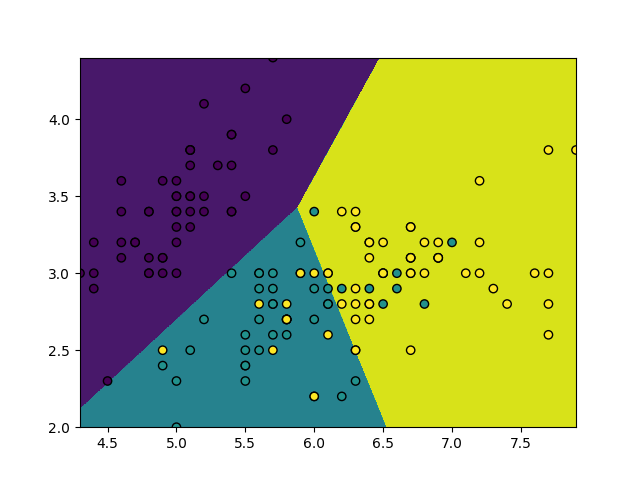
\includegraphics[width = 15 cm ]{Images/ClasificadorLogistico.png}
  \caption{Regiones de clasificación para regresión logística de la base de datos Iris para los sépalos de tres clases diferentes de plantas. }
\end{figure}

Notemos que las fronteras son efectivmente lineales, como se provo en un ejercicio previo. Además vemos que el ajuste con las clases en morado son excelentes, sin embargo ahí donde las clases se junta (amarillo y azul) tenemos clasificadores erroneos.

Finalmente para probar la precisión del modelo, consideremos el comando
\begin{lstlisting}
score = logisticRegr.score(x_test, y_test)
print("Proporción de veces que acierta el modelo: ", score)
\end{lstlisting}
que nos dice la proporción de datos bien clasificados contra el número total de datos. Vemos que al ejecutar el script para la partición de prueba del 20\% tenemos que hay 73.333 \% de datos bien clasificados, es decir 110 datos de los 150 clasifico el modelo de manera asertiva. Luego 40 de los 150 fueron erroenos.


El \textbf{enlace al código} con los detalles del ejercicio práctico se encuentra \href{https://colab.research.google.com/drive/13hEX_ubDx0vYYG6S1ndCaer41euqlr3x?usp=sharing}{\color{blue} aquí}.

\end{document}